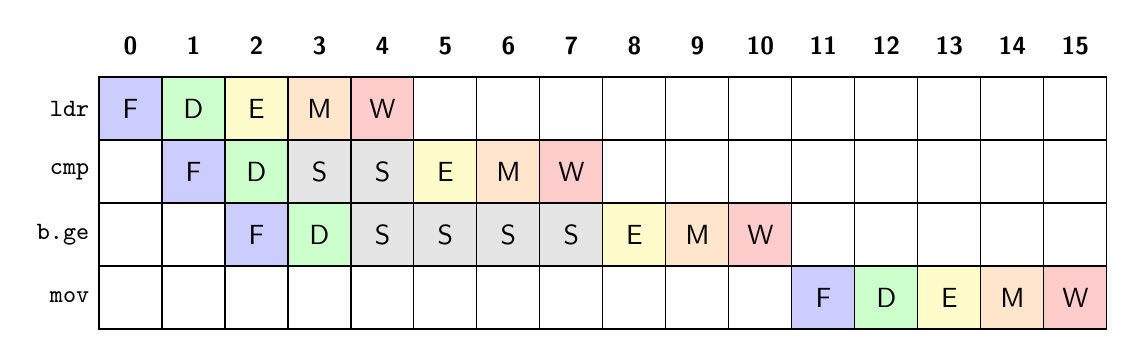
\begin{tikzpicture}[font=\sffamily, scale=0.8]
% Define styles for pipeline stages
\tikzstyle{F} = [fill=blue!20, draw=black, rectangle, minimum width=1cm, minimum height=0.8cm]
\tikzstyle{D} = [fill=green!20, draw=black, rectangle, minimum width=1cm, minimum height=0.8cm]
\tikzstyle{E} = [fill=yellow!20, draw=black, rectangle, minimum width=1cm, minimum height=0.8cm]
\tikzstyle{M} = [fill=orange!20, draw=black, rectangle, minimum width=1cm, minimum height=0.8cm]
\tikzstyle{W} = [fill=red!20, draw=black, rectangle, minimum width=1cm, minimum height=0.8cm]
\tikzstyle{S} = [fill=gray!20, draw=black, rectangle, minimum width=1cm, minimum height=0.8cm]

% Define the number of cycles and instructions
\def\numcycles{15}
\def\numinstr{4}

% Draw the grid
\foreach \i in {1,...,\numinstr} {
    \foreach \j in {0,...,\numcycles} {
        \draw (\j,-\i) rectangle (\j+1,-\i+1);
    }
}

% Label cycles at the top
\foreach \j in {0,...,\numcycles} {
    \node at (\j+0.5,0.5) {\small\textbf{\j}};
}

% Label instructions on the left
\node[anchor=east] at (0,-0.5) {\small \texttt{ldr}};
\node[anchor=east] at (0,-1.5) {\small \texttt{cmp}};
\node[anchor=east] at (0,-2.5) {\small \texttt{b.ge}};
\node[anchor=east] at (0,-3.5) {\small \texttt{mov}};

% Fill in the pipeline stages for each instruction

% Instruction 1 (ldr)
\draw[F] (0,-1) rectangle +(1,1) node[pos=.5] {F};
\draw[D] (1,-1) rectangle +(1,1) node[pos=.5] {D};
\draw[E] (2,-1) rectangle +(1,1) node[pos=.5] {E};
\draw[M] (3,-1) rectangle +(1,1) node[pos=.5] {M};
\draw[W] (4,-1) rectangle +(1,1) node[pos=.5] {W};

% Instruction 2 (cmp)
\draw[F] (1,-2) rectangle +(1,1) node[pos=.5] {F};
\draw[D] (2,-2) rectangle +(1,1) node[pos=.5] {D};
\draw[S] (3,-2) rectangle +(1,1) node[pos=.5] {S};
\draw[S] (4,-2) rectangle +(1,1) node[pos=.5] {S};
\draw[E] (5,-2) rectangle +(1,1) node[pos=.5] {E};
\draw[M] (6,-2) rectangle +(1,1) node[pos=.5] {M};
\draw[W] (7,-2) rectangle +(1,1) node[pos=.5] {W};

% Instruction 3 (b.ge)
\draw[F] (2,-3) rectangle +(1,1) node[pos=.5] {F};
\draw[D] (3,-3) rectangle +(1,1) node[pos=.5] {D};
\draw[S] (4,-3) rectangle +(1,1) node[pos=.5] {S};
\draw[S] (5,-3) rectangle +(1,1) node[pos=.5] {S};
\draw[S] (6,-3) rectangle +(1,1) node[pos=.5] {S};
\draw[S] (7,-3) rectangle +(1,1) node[pos=.5] {S};
\draw[E] (8,-3) rectangle +(1,1) node[pos=.5] {E};
\draw[M] (9,-3) rectangle +(1,1) node[pos=.5] {M};
\draw[W] (10,-3) rectangle +(1,1) node[pos=.5] {W};


% Instruction 4 (mov w0, #0)
\draw[F] (11,-4) rectangle +(1,1) node[pos=.5] {F};
\draw[D] (12,-4) rectangle +(1,1) node[pos=.5] {D};
\draw[E] (13,-4) rectangle +(1,1) node[pos=.5] {E};
\draw[M] (14,-4) rectangle +(1,1) node[pos=.5] {M};
\draw[W] (15,-4) rectangle +(1,1) node[pos=.5] {W};

% % Add legends for pipeline stages
% \matrix [draw, below right] at (14,-0.5) {
%   \node [F] {F}; & \node [anchor=west] {Fetch}; \\
%   \node [D] {D}; & \node [anchor=west] {Decode}; \\
%   \node [E] {E}; & \node [anchor=west] {Execute}; \\
%   \node [M] {M}; & \node [anchor=west] {Memory}; \\
%   \node [W] {W}; & \node [anchor=west] {Write Back}; \\
%   \node [S] {S}; & \node [anchor=west] {Stall}; \\
% };

\end{tikzpicture}
